\documentclass[border=10pt]{standalone}
\usepackage{tikz}
\usetikzlibrary{positioning, arrows.meta, shapes, backgrounds, fit}

\begin{document}
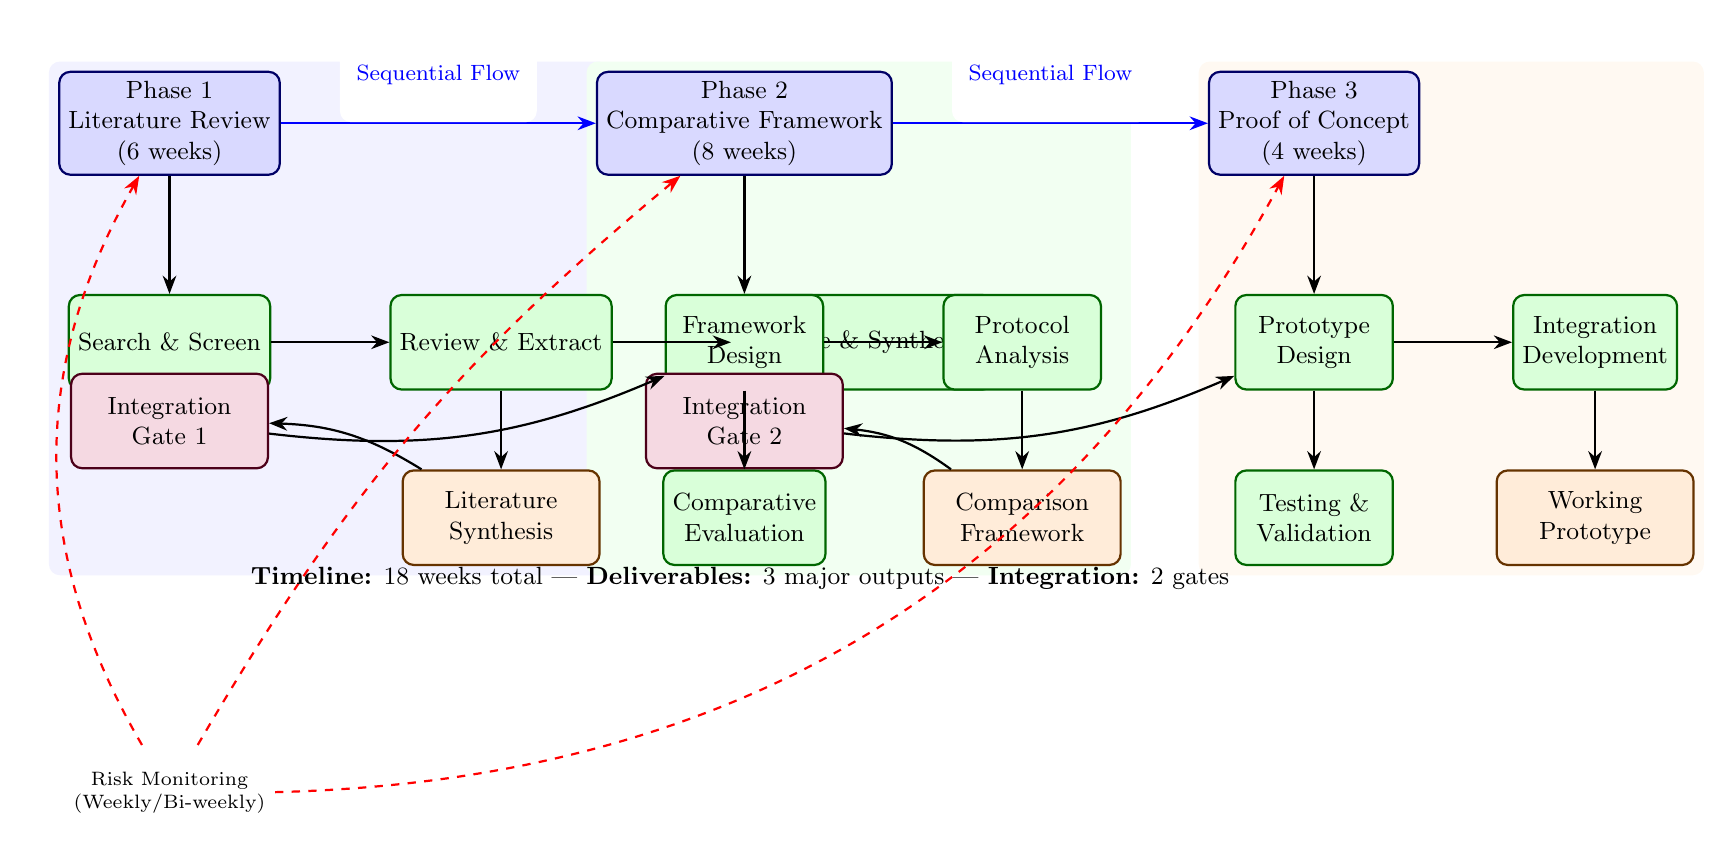
\begin{tikzpicture}[
    node distance=2.5cm and 3.5cm,
    every node/.style={rounded corners, minimum width=2.5cm, minimum height=1.2cm, align=center, font=\small},
    phase/.style={fill=blue!15, draw=blue!40!black, thick},
    activity/.style={fill=green!15, draw=green!40!black, thick, minimum width=2cm},
    output/.style={fill=orange!15, draw=orange!40!black, thick},
    integration/.style={fill=purple!15, draw=purple!40!black, thick},
    arrow/.style={-Stealth, thick},
    dasharrow/.style={-Stealth, thick, dashed},
    label/.style={font=\footnotesize, fill=white, inner sep=2pt}
]

% Phase 1: Literature Review
\node[phase] (phase1) {Phase 1\\Literature Review\\(6 weeks)};
\node[activity, below=1.5cm of phase1] (p1act1) {Search \& Screen};
\node[activity, right=1.5cm of p1act1] (p1act2) {Review \& Extract};
\node[activity, right=1.5cm of p1act2] (p1act3) {Analyze \& Synthesize};
\node[output, below=1cm of p1act2] (p1out) {Literature\\Synthesis};

% Phase 2: Comparative Framework
\node[phase, right=4cm of phase1] (phase2) {Phase 2\\Comparative Framework\\(8 weeks)};
\node[activity, below=1.5cm of phase2] (p2act1) {Framework\\Design};
\node[activity, right=1.5cm of p2act1] (p2act2) {Protocol\\Analysis};
\node[activity, below=1cm of p2act1] (p2act3) {Comparative\\Evaluation};
\node[output, below=1cm of p2act2] (p2out) {Comparison\\Framework};

% Phase 3: Proof of Concept
\node[phase, right=4cm of phase2] (phase3) {Phase 3\\Proof of Concept\\(4 weeks)};
\node[activity, below=1.5cm of phase3] (p3act1) {Prototype\\Design};
\node[activity, right=1.5cm of p3act1] (p3act2) {Integration\\Development};
\node[activity, below=1cm of p3act1] (p3act3) {Testing \&\\Validation};
\node[output, below=1cm of p3act2] (p3out) {Working\\Prototype};

% Integration points
\node[integration, below=2.5cm of phase1] (int1) {Integration\\Gate 1};
\node[integration, below=2.5cm of phase2] (int2) {Integration\\Gate 2};

% Phase connections
\draw[arrow] (phase1) -- (p1act1);
\draw[arrow] (p1act1) -- (p1act2);
\draw[arrow] (p1act2) -- (p1act3);
\draw[arrow] (p1act2) -- (p1out);

\draw[arrow] (phase2) -- (p2act1);
\draw[arrow] (p2act1) -- (p2act2);
\draw[arrow] (p2act1) -- (p2act3);
\draw[arrow] (p2act2) -- (p2out);

\draw[arrow] (phase3) -- (p3act1);
\draw[arrow] (p3act1) -- (p3act2);
\draw[arrow] (p3act1) -- (p3act3);
\draw[arrow] (p3act2) -- (p3out);

% Integration flows
\draw[arrow] (p1out) to[bend right=15] (int1);
\draw[arrow] (int1) to[bend right=15] (p2act1);
\draw[arrow] (p2out) to[bend right=15] (int2);
\draw[arrow] (int2) to[bend right=15] (p3act1);

% Phase-to-phase progression
\draw[arrow, thick, blue] (phase1) -- node[label, above] {Sequential Flow} (phase2);
\draw[arrow, thick, blue] (phase2) -- node[label, above] {Sequential Flow} (phase3);

% Risk monitoring (background process)
\node[below=3.5cm of int1, font=\scriptsize, align=center] (risk) {Risk Monitoring\\(Weekly/Bi-weekly)};
\draw[dasharrow, red] (risk) to[bend left=30] (phase1);
\draw[dasharrow, red] (risk) to[bend left=10] (phase2);
\draw[dasharrow, red] (risk) to[bend right=30] (phase3);

% Background grouping
\begin{scope}[on background layer]
    \node[fit=(phase1) (p1out) (int1), fill=blue!5, rounded corners] {};
    \node[fit=(phase2) (p2out) (int2), fill=green!5, rounded corners] {};
    \node[fit=(phase3) (p3out), fill=orange!5, rounded corners] {};
\end{scope}

% Timeline indicator
\node[below=4.5cm of phase2, font=\small, align=center] {
    \textbf{Timeline:} 18 weeks total | \textbf{Deliverables:} 3 major outputs | \textbf{Integration:} 2 gates
};

\end{tikzpicture}
\end{document}